\documentclass[tikz,border=5pt]{standalone}

\begin{document}

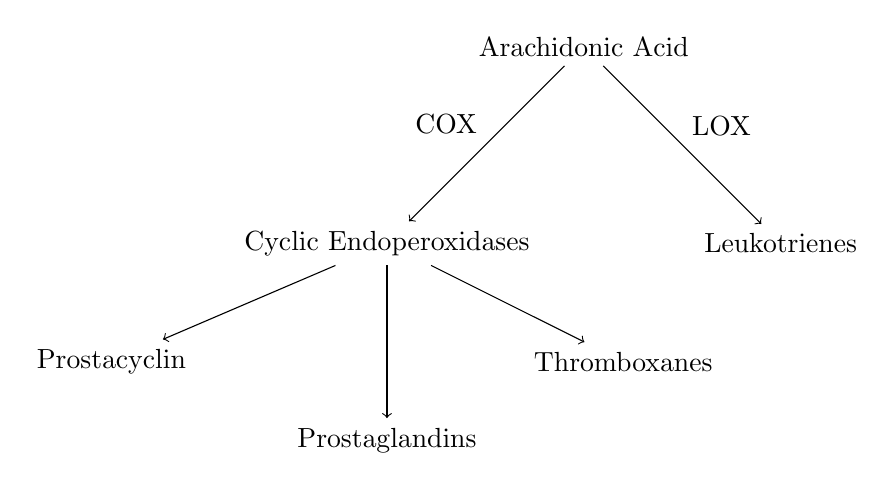
\begin{tikzpicture}[node distance=2cm]

% nodes
\node (A) at (0, 0) {Arachidonic Acid};
\node (B) at (-2.5, -2.5) {Cyclic Endoperoxidases};
\node (C) at (2.5, -2.5) {Leukotrienes};

\node (D) at (0.5,-4) {Thromboxanes};
\node (E) at (-2.5,-5) {Prostaglandins};
\node (F) at (-6,-4) {Prostacyclin};

% arrows
\draw[->, black] (A) -> node[black, above left]{COX}(B);
\draw[->, black] (A) -> node[black, above right]{LOX} (C);

\draw[->, black] (B) -> (D);
\draw[->, black] (B) -> (E);
\draw[->, black] (B) -> (F);

\end{tikzpicture}

\end{document}